\chapter{Experiments and Results}
\label{chapter:experiments}

experiments... \todo{Finish experiments and results}

The code is available at \url{https://github.com/moisestg/rare-lm}.

Maybe mention implementation detail of only calculating $p(y(t))$ when training?

When showing the PSMM mention the initialization of $\mathbf{s}$ and the issue with the gradient.

\begin{table}[]
	\centering
	\begin{tabular}{cc|c|c|c|c|}
		\cline{3-6}
		\multicolumn{1}{l}{}                                                    & \multicolumn{1}{l|}{}   & \multicolumn{2}{c|}{All} & \multicolumn{2}{c|}{Names} \\ \cline{3-6} 
		&                         & Train       & Dev        & Train        & Dev         \\ \hline
		\multicolumn{1}{|c|}{\multirow{2}{*}{Basic}}                            & Baseline                & 42.5        & 61.5       & 1000         & 130K        \\ \cline{2-6} 
		\multicolumn{1}{|c|}{}                                                  & Mixture ($\lambda=100$) & 55          & 69         & 4000         & 120K        \\ \hline
		\multicolumn{1}{|c|}{\multirow{2}{*}{Input dropout}}                    & Baseline                & 52.5        & 63         & 2000         & 140K        \\ \cline{2-6} 
		\multicolumn{1}{|c|}{}                                                  & Mixture ($\lambda=100$) & 65          & 72         & 8000         & 120K        \\ \hline
		\multicolumn{1}{|c|}{\multirow{2}{*}{State dropout}}                    & Baseline                & 48          & 62.5       & 1000         & 120K        \\ \cline{2-6} 
		\multicolumn{1}{|c|}{}                                                  & Mixture ($\lambda=100$) & 62.5        & 73         & 6000         & 120K        \\ \hline
		\multicolumn{1}{|c|}{\multirow{2}{*}{Output dropout}}                   & Baseline                & 62.5        & 65         & 5000         & 150K        \\ \cline{2-6} 
		\multicolumn{1}{|c|}{}                                                  & Mixture ($\lambda=100$) & 80          & 73         & 20K          & 80K         \\ \hline
		\multicolumn{1}{|c|}{\multirow{2}{*}{L2 regularization ($\beta=0.01$)}} & Baseline                & 100         & 125        & 10K          & 400K        \\ \cline{2-6} 
		\multicolumn{1}{|c|}{}                                                  & Mixture ($\lambda=100$) & 107.5       & 119        & 8000         & 120K        \\ \hline
	\end{tabular}
	\caption{Perplexity}
	\label{smmExps}
\end{table}

\begin{figure}[H]
	\centering
	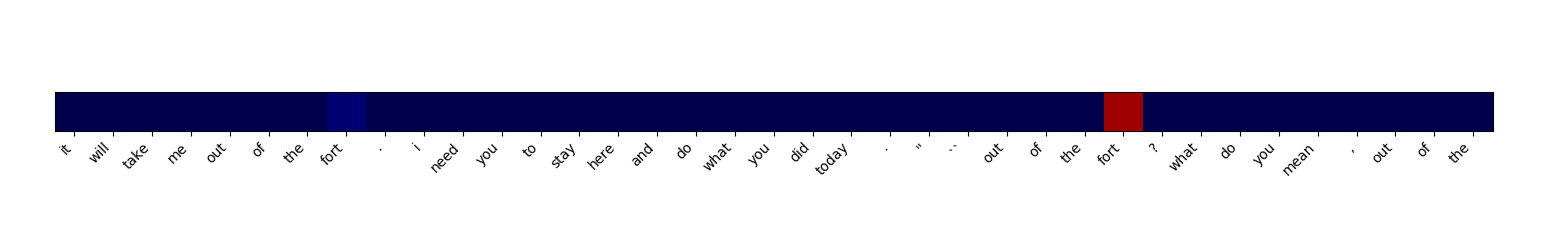
\includegraphics[scale=0.6]{gateEx1}
	\captionof{figure}{Predicting ``fort'' ($g_t=0.28$).}
	\label{fig:gateEx1}
\end{figure}


\begin{table}[]
	\centering
	\begin{tabular}{c|c|c|c|}
		\cline{2-4}
		\multicolumn{1}{l|}{}                             & \textbf{Control} & \textbf{Dev} & \textbf{Test} \\ \hline
		\multicolumn{1}{|c|}{\textbf{PSMM (length=100)}}  & 114.4            & 151.3        & 156.6         \\ \hline
		\multicolumn{1}{|c|}{\textbf{PSMM (length=200)*}} &                  &              &               \\ \hline
		\multicolumn{1}{|c|}{\textbf{PSMM (length=500)*}} &                  &              &               \\ \hline
	\end{tabular}
	\caption{Perplexity on LAMBADA}
	\label{psmmExps}
\end{table}